\documentclass{article}

\usepackage{url}

\usepackage{amssymb,amsfonts,amsmath,amsthm,mathtools}
\usepackage{adjustbox}
\usepackage{float}
\usepackage{caption}
\usepackage{mdframed}
\usepackage{lmodern}
\usepackage{bm,bbold}
\usepackage{xfrac, nicefrac}
\usepackage{lmodern}
\usepackage{enumitem}
\usepackage[margin=60pt]{geometry}

\usepackage{pgfplots, pgf,tikz}
\usepgfplotslibrary{fillbetween}
\pdfinclusioncopyfonts=1
\captionsetup{width=0.85\textwidth}

\usepackage{xcolor}
\definecolor{RED}{HTML}{EB6231}
\definecolor{YELLOW}{HTML}{E29D26}
\definecolor{BLUE}{HTML}{5D80B4}
\definecolor{LIGHTGREEN}{HTML}{6ABD9B}
\definecolor{GREEN}{HTML}{8FB03E}
\definecolor{PURPLE}{HTML}{BE1E2D}
\definecolor{BROWN}{HTML}{A97C50}
\definecolor{PINK}{HTML}{DA1C5C}

\newcommand{\specialcell}[2][c]{%
	\begin{tabular}[#1]{@{}c@{}}#2\end{tabular}}

\DeclareMathOperator{\E}{\mathbb{E}}
\newcommand{\der}{\mathrm{d}}
\newcommand{\e}{\mathrm{e}}
\newcommand{\angstrom}{\text{\normalfont\AA}}

% Time, effective population size and mutation rate.
\newcommand{\Ne}{N_{\mathrm{e}}}
\newcommand{\dnds}{\omega}
\newcommand{\Nsite}{\text{n}}
\newcommand{\site}{\text{i}}
\newcommand{\Nstate}{\text{K}}

\newcommand{\x}{x}
\newcommand{\eq}{^{*}}
\newcommand{\dx}{\delta \x}
\newcommand{\s}{s}
\newcommand{\deltaG}{\Delta G}
\newcommand{\deltaGMin}{\alpha}
\newcommand{\deltadeltaG}{\Delta \deltaG}

\newcommand{\ci}{\mathbb{S}_{t}}
\newcommand{\cj}{\mathbb{S}_{t}'}
\newcommand{\itoj}{\ci, \cj}
\newcommand{\setNeighbors}{\mathcal{M}\left(\ci\right)}
\newcommand{\setNonSynNeighbors}{\mathcal{N}\left(\ci\right)}
\newcommand{\setSynNeighbors}{\mathcal{S}\left(\ci\right)}
\newcommand{\submatrix}{q}


\begin{document}
\part*{Supplementary materials}

\section*{Genotype to phenotype map}
Define $\Nsite$ as the number of sites in the genotype sequence.
Each site can be in one of $\Nstate \geq 2$ states, where only $1$ state is defined the stable state, and $\Nstate - 1$ states are unstable.
For a given genotype sequence, define phenotype $0 \leq \x \leq 1$ as the current proportion of sites in the unstable state.
After a mutation, given that only one site can change at a time, the absolute change of $\x$ is either $0$ or $\dx=\sfrac{1}{\Nsite}$.
Define $\rho_{\x}(\dx)$ as the probability to get a change of phenotype equal to $\dx$, if the current phenotype is $\x$:\\
\begin{gather}
\begin{cases}
\dx &\text{ with probability } \rho_{\x}(\dx) = 1-x, \\
0 &\text{ with probability } \rho_{\x}(0) = \x \left[1 - \frac{1}{\Nstate - 1}\right], \\
-\dx &\text{ with probability } \rho_{\x}(-\dx) = \frac{\x}{\Nstate - 1}.\\
\end{cases} \label{eq:proba}
\end{gather}

\section*{Selection coefficient}
$s(\x, \dx)$ is the selection coefficient of an effect $\dx$ if the current phenotype is $\x$:
\begin{align}
s(\x, \dx) &= \frac{f(\x + \dx) - f(\x)}{f( \x)}, \\
 &\simeq \frac{1}{f(\x)}\frac{\der f( \x)}{\der \x} \dx, \\
 &\simeq \frac{\der \ln (f(\x))}{\der \x} \dx, \label{eq:s_from_fitness}
\end{align}
where $f( \x)$ is the Wrightian fitness of phenotype $x$. And thus we also have:
\begin{gather}
s(\x, -\dx) \simeq - s(\x, \dx) \text{ from eq. \ref{eq:s_from_fitness}} \label{eq:s_minus_deltax}, \\
\iff S(\x, -\dx) \simeq - S(\x, \dx), \label{eq:S_minus_deltax}
\end{gather}
where $S(\x\eq, \dx) = 4\Ne s (\x\eq, \dx)$ is the scaled selection coefficient.

\section*{Probability of fixation}
The probability of fixation of a mutation with effect $\dx$, for a resident phenotype $\x$ is :
\begin{align}
p_{\text{fix}}(\x, \dx) &= \frac{ 2 s(\x, \dx)}{1 - \e^{-4\Ne s(\x, \dx)}}, \\
 &= \frac{ 2 s(\x, \dx)}{1 - \e^{-S(\x, \dx)}}. \label{eq:pfix}
\end{align}
And in the case of neutral mutations, the probability of fixation is:
\begin{gather}
p_{\text{fix}}(\x, 0) = \frac{ 1}{2 \Ne} \label{eq:pfix0}.
\end{gather}
And the ratio of probability of fixation between selected and neutral mutations is:
\begin{align}
\frac{p_{\text{fix}}(\x, \dx)}{p_{\text{fix}}(\x, 0)} & = \frac{ 2 \Ne 2 s(\x, \dx)}{1 - \e^{-S(\x, \dx)}} \text{ from eq. \ref{eq:pfix} and \ref{eq:pfix0}},\\
& = \frac{S(\x, \dx)}{1 - \e^{-S(\x, \dx)}} \label{eq:pfixratio}.
\end{align}
\section*{Equilibrium phenotype}
At equilibrium phenotype $\x\eq$, the expected selection coefficient of mutation that reached fixation must be $0$:
\begin{gather}
 0 = \E_{\dx} \left[ s(\x\eq, \dx) p_{\text{fix}}(\x\eq, \dx) \right], \\
\iff 0 = \frac{ 2 s(\x\eq, \dx)^2}{1 - \e^{-S(\x\eq, \dx)}}   \rho_{\x\eq}(\dx) + s(\x\eq, 0) \frac{ \rho_{\x\eq}(0)}{2\Ne} + \frac{ 2s(\x\eq, -\dx)^2}{1 - \e^{-S(\x\eq, -\dx)}} \rho_{\x\eq}(-\dx)\text{ from eq. \ref{eq:pfix} and \ref{eq:pfix0}}, \\
\Longrightarrow \frac{ 2s(\x\eq, \dx)^2}{1 - \e^{-S(\x\eq, \dx)}}   \rho_{\x\eq}(\dx) \simeq \frac{ - 2s(\x\eq, \dx)^2}{1 - \e^{S(\x\eq, \dx)}}   \rho_{\x\eq}(-\dx) \text{ from eq. \ref{eq:S_minus_deltax}}, \\
\iff \frac{ \rho_{\x\eq}(\dx)}{\rho_{\x\eq}(-\dx)} \simeq \e^{-S(\x\eq, \dx)} \frac{ \e^{-S(\x\eq, \dx)} - 1}{ \e^{-S(\x\eq, \dx)} \left( 1 - \e^{S(\x\eq, \dx)} \right)}, \\
\iff \ln \left( \frac{1 - \x\eq}{\x\eq} \right) + \ln (\Nstate-1) \simeq -S(\x\eq, \dx) \text{ from eq. \ref{eq:proba}} \label{eq:equilibrium}, \\
\iff \lambda_{K}(\x\eq) \simeq -S(\x\eq, \dx) \label{eq:equilibrium_lambda},
\end{gather}
where  $\lambda_{K}(\x\eq) = \ln \left( \frac{1 - \x\eq}{\x\eq} \right) + \ln (\Nstate-1)$.
\section*{Substitution rate ($\bm{\dnds}$) at equilibrium}
The substitution rate of selected mutations relative to neutral mutations  ($\dnds$) is by definition:
\begin{align}
\dnds & = \E_{\dx} \left[ \frac{p_{\text{fix}}(\x, \dx)}{p_{\text{fix}}(\x, 0)} \right], \\
 & = (1 - \x) \frac{ S(\x, \dx)}{1 - \e^{-S(\x, \dx)}} + \x \left(\frac{\Nstate - 2}{\Nstate - 1}\right) + \frac{\x}{\Nstate-1} \frac{ S(\x, -\dx)}{1 - \e^{-S(\x, -\dx)}} \text{ from eq. \ref{eq:proba}, \ref{eq:pfix} and \ref{eq:pfix0}}, \\
 & = (1 - \x) \frac{ S(\x, \dx)}{1 - \e^{-S(\x, \dx)}} - \frac{\x}{\Nstate-1}  \frac{ S(\x, \dx)}{1 - \e^{S(\x, \dx)}} +  \x \left(\frac{\Nstate - 2}{\Nstate - 1}\right) \text{ from eq. \ref{eq:S_minus_deltax}}.
\end{align}
$\dnds\eq$ at equilibrium is then determined by the phenotype at equilibrium $\x\eq$:
\begin{align}
\dnds\eq &= (1 - \x\eq) \frac{ S(\x\eq, \dx)}{1 - \e^{-S(\x\eq, \dx)}} - \frac{\x\eq}{\Nstate-1} \frac{ S(\x\eq, \dx)}{1 - \e^{S(\x\eq, \dx)}} + \x\eq \left(\frac{\Nstate - 2}{\Nstate - 1}\right) , \\
 &= \x\eq \left[ \frac{2 (\x\eq-1)  \lambda_{K}(\x\eq) }{\Nstate (\x\eq-1)+1} + \frac{\Nstate - 2}{\Nstate - 1}\right] \text{ from eq. \ref{eq:equilibrium}}.
\end{align}
\begin{center}
	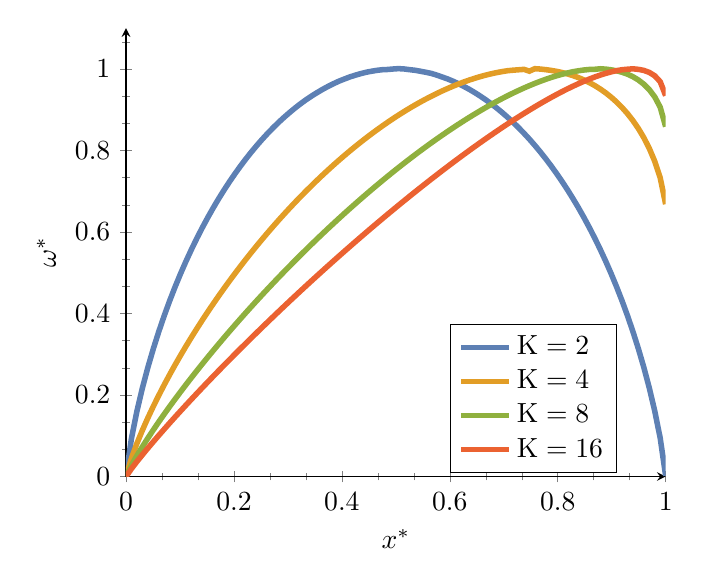
\begin{tikzpicture}[
	declare function={
		omega(\x,\k)= \x*(2*(\x-1)*(ln(\k-1)+ln((1-\x)/\x))/(\k*(\x-1)+1)+ (\k-2)/(\k-1));
	},]
	\begin{axis}[
	ylabel={$\dnds\eq$},
	xlabel={$\x\eq$},
	domain=0:1.0,
	ymin=0.0, ymax=1.1,
	samples=100,
	legend entries={$\Nstate=2$, $\Nstate=4$, $\Nstate=8$, $\Nstate=16$},
	legend cell align=left,
	minor tick num=2,
	axis x line=bottom,
	axis y line=left,
	legend style={at={(0.6,0.34)},anchor=north west}
	]
	\addplot[line width=2.0pt, color=BLUE]{omega(x, 2)};
	\addplot[line width=2.0pt, color=YELLOW]{omega(x, 4)};
	\addplot[line width=2.0pt, color=GREEN]{omega(x, 8)};
	\addplot[line width=2.0pt, color=RED]{omega(x, 16)};
	\end{axis}
	\end{tikzpicture}
\end{center}
And the derivative of $\dnds\eq$ w.r.t to $\x\eq$ is: 
\begin{gather}
\frac{\der \dnds\eq}{\der \x\eq} = 2 \left[ \frac{\Nstate (\x\eq- 1) + 1+\left[\Nstate (\x\eq-1)^2+2 \x\eq-1\right] \lambda_{K}(\x\eq) }{(\Nstate (\x\eq-1)+1)^2}\right] + \frac{\Nstate - 2}{\Nstate - 1} \label{eq:dw_dx}.
\end{gather}
\begin{center}
	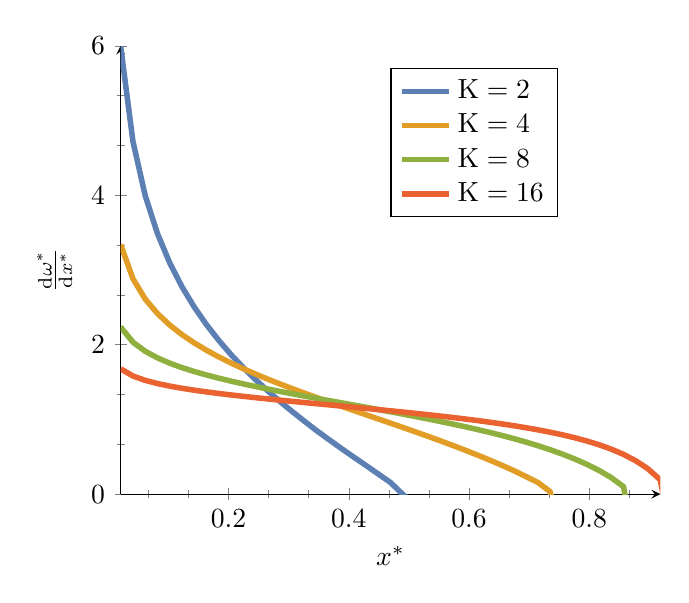
\begin{tikzpicture}[
	declare function={
		domega(\x,\k)= 2*(\k*(\x-1)+1 + (\k*(\x-1)^2+2*\x-1)*(ln(\k-1) + ln((1-\x)/\x)))/(\k*(\x - 1) + 1)^2 + (\k-2) / (\k-1);
	},]
	\begin{axis}[
	ylabel={$\frac{\der \dnds\eq}{\der \x\eq}$},
	xlabel={$\x\eq$},
	domain=0.0:1.0,
	ymin=0, ymax=6,
	samples=50,
	legend entries={$\Nstate=2$, $\Nstate=4$, $\Nstate=8$, $\Nstate=16$},
	legend cell align=left,
	minor tick num=2,
	axis x line=bottom,
	axis y line=left,
	legend style={at={(0.5,0.95)},anchor=north west}
	]
	\addplot[line width=2.0pt, color=BLUE]{domega(x, 2)};
	\addplot[line width=2.0pt, color=YELLOW]{domega(x, 4)};
	\addplot[line width=2.0pt, color=GREEN]{domega(x, 8)};
	\addplot[line width=2.0pt, color=RED]{domega(x, 16)};
	\end{axis}
	\end{tikzpicture}
\end{center}

\section*{Response of equilibrium after a change in $\bm{\Ne}$}
Define the function $G(\x, \Ne )$ as:
\begin{gather}
G(\x, \Ne ) \equiv \ln \left( \frac{1 - \x}{\x} \right) + \ln (\Nstate-1) + 4 \Ne s(\x, \dx), 
\end{gather}
The equilibrium equation (eq. \ref{eq:equilibrium}) states that $G(\x\eq, \Ne )=0$, meaning that $\x\eq$ is implicitly a function of $\Ne$:
\begin{gather}
G(\x\eq(\Ne), \Ne ) = 0, \\
\Longrightarrow \frac{\partial G(\x\eq, \Ne ) }{\partial \x\eq }\frac{ \der \x\eq}{\der \Ne} + \frac{ \partial G(\x\eq, \Ne )}{\partial \Ne} = 0, \\
\iff \left[ \frac{\partial \ln (1-\x\eq) }{\partial \x\eq } - \frac{\partial \ln (\x\eq) }{\partial \x\eq}  + 4 \Ne \frac{ \partial s(\x\eq, \dx) }{\partial \x\eq } \right]\frac{ \der \x\eq}{\der \Ne} + 4 s(\x\eq, \dx) = 0, \\
\iff \left[ \frac{1}{(1 - \x\eq) \x\eq} + 4 \Ne \frac{ \partial^2 \ln f(\x\eq) }{\partial {\x\eq}^2}\dx \right]\frac{ \der \x\eq}{\der \Ne}  = - 4 \frac{ \partial \ln f(\x\eq) }{\partial {\x\eq}}\dx \text{ from eq. \ref{eq:s_from_fitness}}, \\
\iff 4 \dx \left[ \frac{1}{4 \dx \Ne  (1 - \x\eq) \x\eq} + \frac{ \partial^2 \ln f(\x\eq) }{\partial {\x\eq}^2} \right] \Ne \frac{ \der \x\eq}{\der \Ne}  = - 4 \dx \frac{ \partial \ln f(\x\eq) }{\partial {\x\eq}}, \\
\iff \frac{ \der \x\eq}{\der \ln (\Ne)}  = - \frac{\frac{ \partial \ln f(\x\eq) }{\partial {\x\eq}}}{\frac{1}{4 \dx \Ne  (1 - \x\eq) \x\eq} + \frac{ \partial^2 \ln f(\x\eq) }{\partial {\x\eq}^2}}  \label{eq:dx_dlnNe}.
\end{gather}
Giving the equation for the response of phenotype at equilibrium after a change of effective population size.
Together, the response of substitution rate at equilibrium, after a change of effective population size can be obtain as:
\begin{align}
\frac{\der \dnds\eq}{\der \ln (\Ne)} & = \frac{\der \dnds\eq}{\der \x\eq} \frac{ \der \x\eq}{\der \ln (\Ne)}, \\
 &= - \frac{\der \dnds\eq}{\der \x\eq} \frac{\frac{ \partial \ln f(\x\eq) }{\partial {\x\eq}}}{\frac{1}{4 \dx \Ne  (1 - \x\eq) \x\eq} + \frac{ \partial^2 \ln f(\x\eq) }{\partial {\x\eq}^2}} \text{ from eq. \ref{eq:dx_dlnNe}} \label{eq:dw_dlnNe}.
\end{align}
\section*{Phenotype to fitness mapping}
From a given phenotype $\x$, define the fitness as :
\begin{gather}
 f(\x) = \frac{1}{1 + \e^{\beta(\deltaGMin + \Nsite \gamma \x)}}, \label{eq:fitness}
\end{gather}
where $\deltaGMin = \Delta G_0 < 0$ is the difference in free energy between stable and unstable protein when all sites are stable. $\Nsite \gamma$ is the expected change in $\Delta G$ when all sites are unstable. By definition, $\Nsite \gamma \dx = \sfrac{\Nsite \gamma}{\Nsite} = \Delta \Delta G $\\
The derivative of fitness w.r.t to phenotype is:
\begin{align}
 \frac{\partial \ln (f(\x))}{\partial \x}  & = - \frac{\partial \ln \left( 1 + \e^{\beta(\deltaGMin + \Nsite \gamma \x)} \right)}{\partial \x} \text{ from eq. \ref{eq:fitness}}, \\
 & = - \beta \Nsite \gamma \frac{\e^{\beta(\deltaGMin + \Nsite \gamma \x)}}{1 + \e^{\beta(\deltaGMin + \Nsite \gamma \x)}} \label{eq:df_dx}.
\end{align}
And the second derivative of fitness w.r.t to phenotype is:
\begin{align}
\frac{\partial^2 \ln (f(\x))}{\partial {\x}^2} & = - \beta \Nsite \gamma \frac{\partial}{\partial \x} \left( \frac{\e^{\beta(\deltaGMin + \Nsite \gamma \x)}}{1 + \e^{\beta(\deltaGMin + \Nsite \gamma \x)}} \right) \text{ from eq. \ref{eq:df_dx}}, \\
 & = - \beta \Nsite \gamma  \beta \Nsite \gamma \frac{\e^{\beta(\deltaGMin + \Nsite \gamma \x)}}{\left( 1 + \e^{\beta(\deltaGMin + \Nsite \gamma \x)}\right)^2}, \\
 & = \frac{\beta \Nsite \gamma}{1 + \e^{\beta(\deltaGMin + \Nsite \gamma \x)}} \frac{ \partial \ln f(\x) }{\partial {\x}} \text{ from eq. \ref{eq:df_dx}} \label{eq:df2_dx2}.
\end{align}
The equilibrium phenotype ($\x\eq$) is :
\begin{gather}
\lambda_{K}(\x\eq) = 4\Ne \beta \gamma \frac{\e^{\beta(\deltaGMin + \Nsite \gamma \x\eq)}}{1 + \e^{\beta(\deltaGMin + \Nsite \gamma \x\eq)}}  \text{ from eq. \ref{eq:equilibrium_lambda} and \ref{eq:df_dx}}.
\end{gather}
Using $\Ne=10^4$, $\beta=1.686$, $\deltaGMin = -118$, $\Nsite=300$, $\gamma=1$, we have the following:
\begin{center}
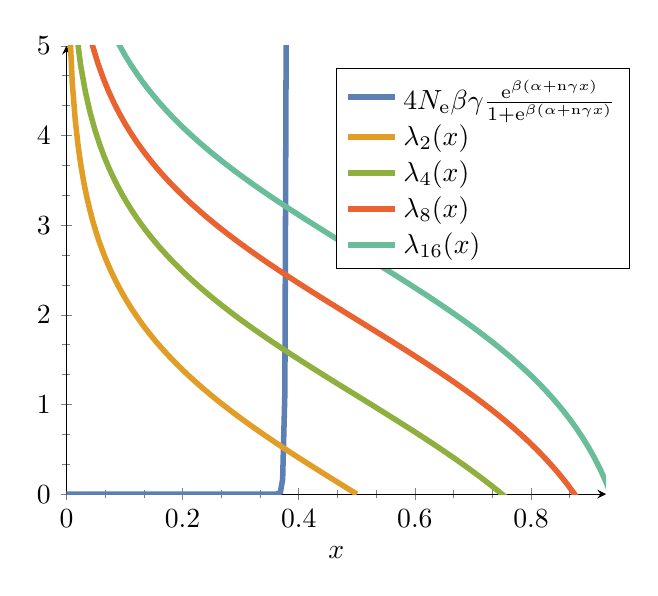
\begin{tikzpicture}[
	declare function={
		lambda(\x,\k)= ln(\k-1) + ln((1-\x)/\x);
	},]
	\begin{axis}[
	xlabel={$\x$},
	ymin=0.0, ymax=5.0,
	samples=100,
	legend entries={
		$4\Ne \beta \gamma \frac{\e^{\beta(\deltaGMin + \Nsite \gamma \x)}}{1 + \e^{\beta(\deltaGMin + \Nsite \gamma \x)}}$,
		$\lambda_{2}(\x)$,
		$\lambda_{4}(\x)$,
		$\lambda_{8}(\x)$,
		$\lambda_{16}(\x)$},
	legend cell align=left,
	minor tick num=2,
	axis x line=bottom,
	axis y line=left,
	legend style={at={(0.5,0.95)},anchor=north west}
	]
	\addplot[domain=0.0:0.38, line width=2.0pt, color=BLUE]{ 4 * 1000 * 1.686 *exp(1.686 * (-118 + 300 *x))};
	\addplot[domain=0.0:0.5,line width=2.0pt, color=YELLOW]{ lambda(x,2) };
	\addplot[domain=0.0:0.8,line width=2.0pt, color=GREEN]{ lambda(x,4) };
	\addplot[domain=0.0:0.9,line width=2.0pt, color=RED]{ lambda(x,8) };
	\addplot[domain=0.0:1.0,line width=2.0pt, color=LIGHTGREEN]{ lambda(x,16) };
	\end{axis}
\end{tikzpicture}
\end{center}
\section*{Approximations}
We assume that $\Ne \gg 1$, $\deltaGMin + \Nsite \gamma \gg 1$ and $ \gamma \simeq 1$.
\begin{gather}
-S(\x\eq, \dx) \simeq \lambda_{\Nstate}(\x\eq)\text{ from eq. \ref{eq:equilibrium_lambda}}, \\
\iff s(\x\eq, \dx) \simeq -\frac{\lambda_{\Nstate}(\x\eq)}{4 \Ne}, \\
\iff \frac{\der \ln (f(\x))}{\der \x} \simeq - \frac{\lambda_{\Nstate}(\x\eq)}{4 \Ne \dx}\text{ from eq. \ref{eq:s_from_fitness}}, \label{eq:approx_df_dx}\\
\iff \beta \Nsite \gamma \frac{\e^{\beta(\deltaGMin + \Nsite \gamma \x)}}{1 + \e^{\beta(\deltaGMin + \Nsite \gamma \x)} } \simeq \frac{\lambda_{\Nstate}(\x\eq)}{4 \Ne \dx}\text{ from eq. \ref{eq:df_dx}}, \\
\iff \frac{\e^{\beta(\deltaGMin + \Nsite \gamma \x)}}{1 + \e^{\beta(\deltaGMin + \Nsite \gamma \x)}} \simeq \frac{\lambda_{\Nstate}(\x\eq)}{4 \Ne \beta \gamma}, \\
\Longrightarrow \frac{\e^{\beta(\deltaGMin + \Nsite \gamma \x)}}{1 + \e^{\beta(\deltaGMin + \Nsite \gamma \x)}} \ll 1\text{ given that $\Ne \gg 1$ and $ \gamma  \simeq 1$}, \\
\Longrightarrow \e^{\beta(\deltaGMin + \Nsite \gamma \x)} \ll 1. \label{eq:approx_exp}
\end{gather}
Moreover, we can get the following:
\begin{gather}
\frac{\der \ln (f(\x))}{\der \x} \simeq - \frac{\lambda_{\Nstate}(\x\eq)}{4 \Ne \dx}\text{ from eq. \ref{eq:approx_df_dx}}, \\
\iff \frac{ \partial^2 \ln f(\x) }{\partial {\x}^2} \simeq - \frac{\lambda_{\Nstate}(\x\eq)}{4 \Ne \dx } \frac{\beta \Nsite \gamma}{1 + \e^{\beta(\deltaGMin + \Nsite \gamma \x)}}\text{ from eq. \ref{eq:df2_dx2}}, \\
\Longrightarrow \frac{ \partial^2 \ln f(\x) }{\partial {\x}^2} \simeq - \frac{\lambda_{\Nstate}(\x\eq)\beta \Nsite \gamma}{4 \Ne \dx  }\text{ from eq. \ref{eq:approx_exp}}, \\
\iff \frac{ \partial^2 \ln f(\x) }{\partial {\x}^2} \simeq - \lambda_{\Nstate}(\x\eq) (1 - \x\eq)\x\eq \beta \Nsite \gamma \frac{1}{4 \dx \Ne  (1 - \x\eq) \x\eq}, \\
\Longrightarrow \left| \frac{ \partial^2 \ln f(\x) }{\partial {\x}^2} \right| \gg \left| \frac{1}{4 \dx \Ne  (1 - \x\eq) \x\eq} \right|\text{ given that $\Nsite \gamma \gg 1$}. \label{eq:approx_df2_df} \\
\end{gather}
Together, these approximations leads to the following response in equilibrium phenotype at change in $\Ne$ as:
\begin{align}
\frac{ \der \x\eq}{\der \ln (\Ne)} & = - \frac{\frac{ \partial \ln f(\x\eq) }{\partial {\x\eq}}}{\frac{1}{4 \dx \Ne  (1 - \x\eq) \x\eq} + \frac{ \partial^2 \ln f(\x\eq) }{\partial {\x\eq}^2}}\text{ from eq. \ref{eq:dw_dlnNe}}, \\
& \simeq - \frac{\frac{ \partial \ln f(\x\eq) }{\partial {\x\eq}}}{\frac{ \partial^2 \ln f(\x\eq) }{\partial {\x\eq}^2}}\text{ from eq. \ref{eq:approx_df2_df}}, \\
& \simeq - \frac{1 + \e^{\beta(\deltaGMin + \Nsite \gamma \x\eq)}}{\beta \Nsite \gamma}\text{ from eq. \ref{eq:df2_dx2}}, \\
& \simeq - \frac{1}{\beta \Nsite \gamma}\text{ from eq. \ref{eq:approx_exp}}. \label{eq:approx_dx_dlnNe}
\end{align}
Moreover, given that the number of state if large enough $\Nstate \gg 1$, the response in equilibrium $\dnds$ due to change in phenotype can be approximated as:
\begin{align}
\frac{ \der \dnds\eq}{\der \x\eq}  & = 2 \left[ \frac{\Nstate (\x\eq- 1) + 1+\left[\Nstate (\x\eq-1)^2+2 \x\eq-1\right] \lambda_{K}(\x\eq) }{(\Nstate (\x\eq-1)+1)^2}\right] + \frac{\Nstate - 2}{\Nstate - 1}\text{ from eq. \ref{eq:approx_exp}}, \\
& \simeq \frac{2 \lambda_{K}(\x\eq)}{\Nstate} + 1, \\
& \simeq 1. \label{eq:approx_domega_dx}
\end{align}
Finally,
\begin{align}
\frac{ \der \dnds\eq}{\der \ln (\Ne)}  & = \frac{ \der \dnds\eq}{\der \x\eq}  \frac{ \der \x\eq}{\der \ln (\Ne)}, \\
  & \simeq - \frac{1}{\beta \Nsite \gamma} \text{from eq. \ref{eq:approx_dx_dlnNe} and \ref{eq:approx_domega_dx}}.
\end{align}


\section*{Probability of folding as in Goldstein \& Pollock}
We simulated substitutions in the protein phosphatase ($\Nsite=300$ codon sites).
From a DNA sequence $\ci$ after $t$ substitutions, we compute the free energy of the folded state $G_{\mathrm{F}}\left(\ci\right)$, using the $3$-dimensional structure of the folded state and pair-wise contact energies between neighboring amino-acid residues:
\begin{equation}
G_{\mathrm{F}}\left(\ci\right) = \sum_{1 \leq \site \leq \Nsite} \sum_{r \in \mathcal{N}(\site)} I \left(\ci(\site), \ci(r) \right),
\end{equation}
where $I(a,b)$ is the pair-wise contact energies between amino-acid $a$ and $b$, using contact potentials estimated by Miya-zawa and Jernigan, and $\mathcal{N}(\site)$ are the neighbor residues of site $\site$ (closer than $7\angstrom$) in the $3$D structure.\\

The free energy of unfolded states $G_{\mathrm{U}}\left(\ci\right)$ is approximated using $55$ decoy $3$D structures that supposedly represent a sample of possible unfolded states:
\begin{equation}
G_{\mathrm{U}}\left(\ci\right) = \langle G\left(\ci\right) \rangle - kT \ln (1.0\mathrm{E}^{160}) - \dfrac{2 \left[ \langle G\left(\ci\right)^2 \rangle - \langle G\left(\ci\right) \rangle^2\right] }{kT}
\end{equation}
where the average $\langle . \rangle$ runs other the $55$ decoy $3$D structures, and $k$ is the Boltzmann constant and $T$ the temperature in Kelvin.\\

From the energy of folded and unfolded states, we can compute the difference in free energy between the states:
\begin{equation}
\deltaG\left(\ci\right) = G_{\mathrm{F}}\left(\ci\right) - G_{\mathrm{U}}\left(\ci\right)
\end{equation}

\begin{center}
	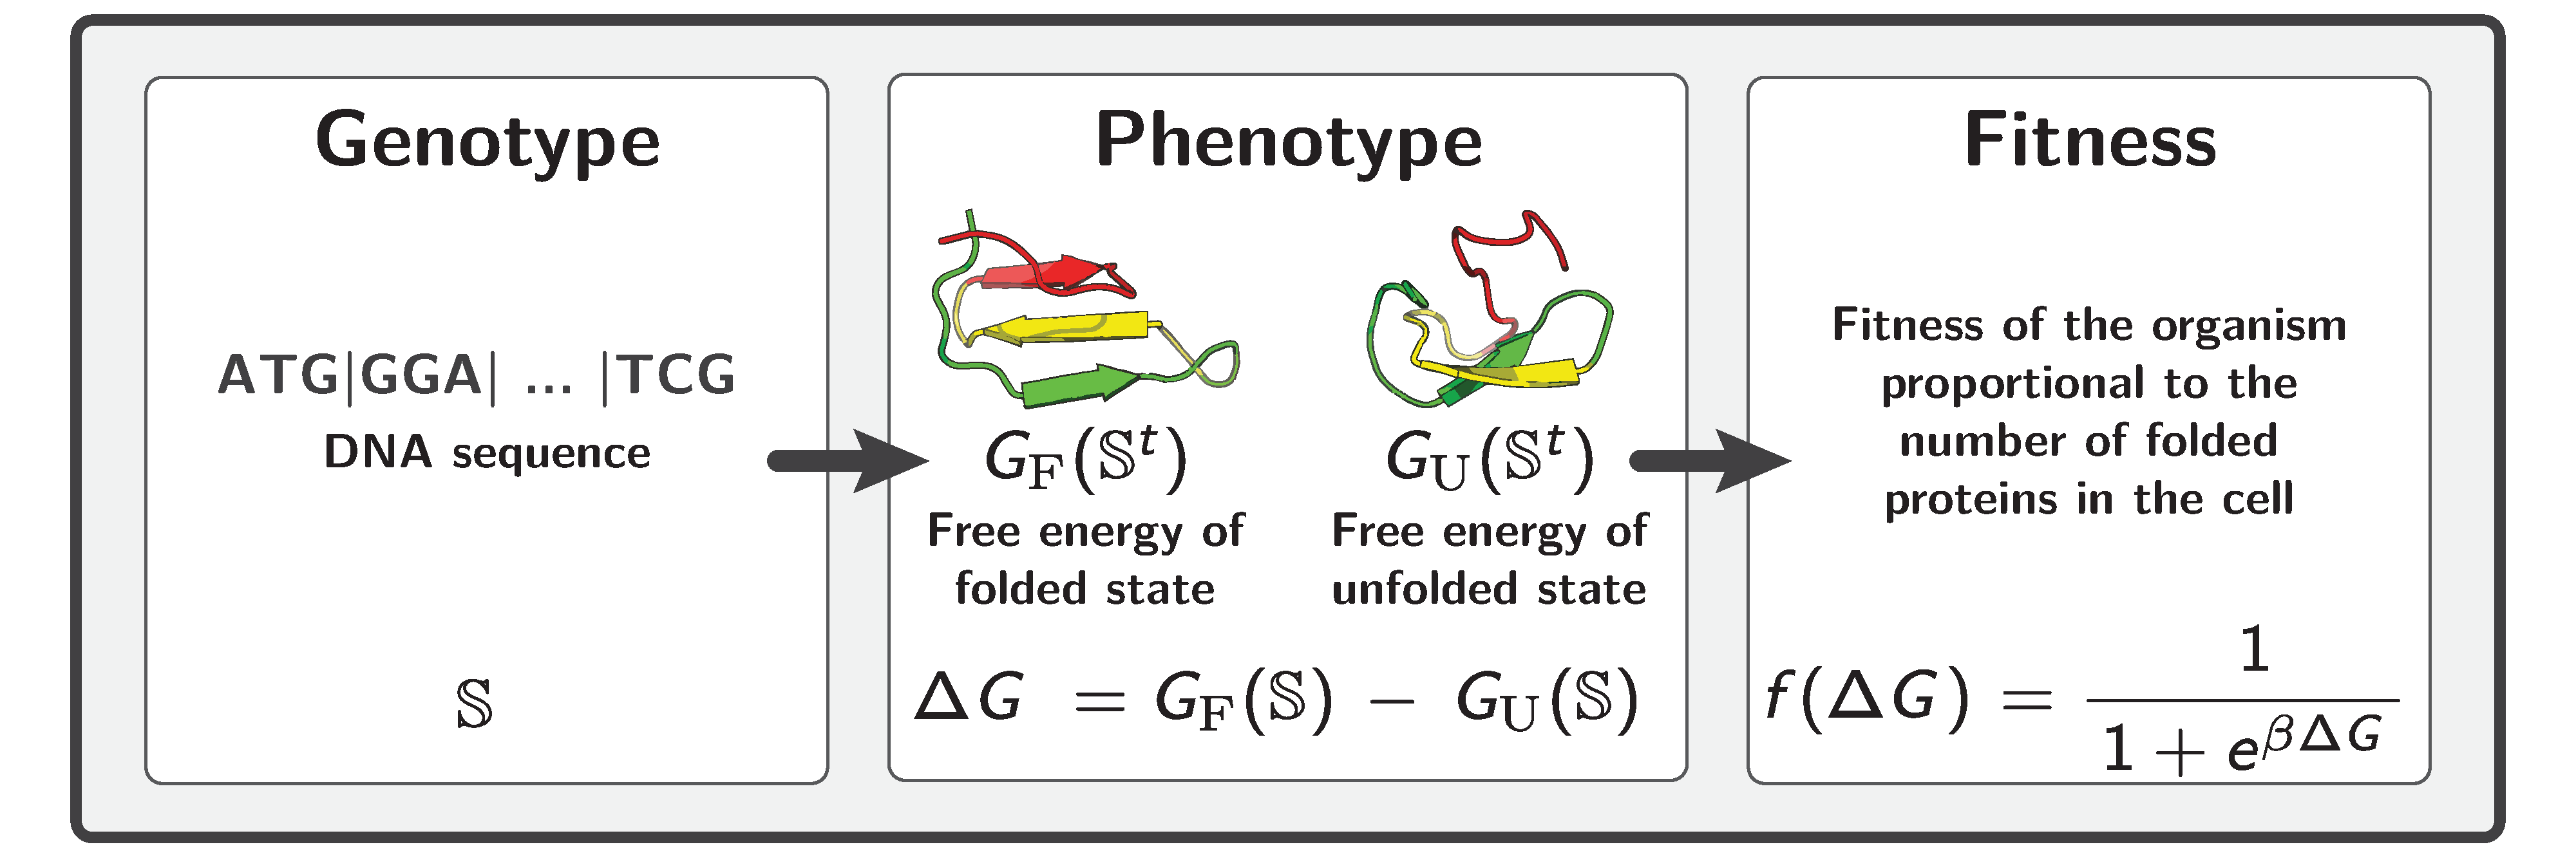
\includegraphics[width=165mm] {artworks/ModelSimuFold.pdf}
\end{center}


\begin{mdframed}
\begin{center}
	\includegraphics[width=0.6\textwidth] {artworks/GoldsteinPollock/sub-DeltaG-mean.pdf}\\
	\textbf{$\bm{\deltaG}$ response to change in $\bm{\Ne}$}.
	$\deltaG$ at equilibrium (blue solid line) is linearly (blue dashed line) dependent on log-$\Ne$, as predicted in the model of Goldstein \& Pollock, with a slope equal to $\beta^{-1}$.
	\label{fig:EqdndsNe}
\end{center}
\end{mdframed}

\section*{Equimutability}
We define $\x$ as the current phenotype and $\dx$ as the phenotypic effect of a mutation.
$\s \left( \x, \dx \right)$ is the selection coefficient of a phenotypic effect $\dx$ if the current phenotype is $\x$:
\begin{equation*}
\s \left( \x, \dx \right) = \dfrac{w \left( \x + \dx \right) - w \left( \x \right)}{w \left( \x \right)} \simeq w'\left( \x \right) \dx, 
\end{equation*}
where $w \left( \x \right)$ is the Wrightian fitness of phenotype $x$.
We also define $\rho_{\x}(\dx)$ as the distribution of phenotypic effects, at phenotype $\x$.
At equilibrium, the expected selection coefficient $ 4 \Ne \s \left( \x, \dx \right)$ of mutations that reached fixation must be $0$:
\begin{align*}
0 & = \E_{\dx} \left[ 4 \Ne \s\left( \x, \dx \right) \dfrac{ 4 \Ne \s\left( \x, \dx \right) }{1 - \e^{4\Ne\s\left( \x, \dx \right)}} \right] \\ & 
\simeq \int_{-\infty}^{\infty} \dfrac{ \left[ 4 \Ne f'\left( \x \right)  \right]^2}{1 - \e^{4\Ne f'\left( \x \right) \dx} }  \dx^2  \rho_{\x}(\dx) \der \dx 
\end{align*}
And the substitution rate is :
\begin{align*}
\omega(\Ne) & = \E_{\dx} \left[ \dfrac{ 4 \Ne \s \left( \x, \dx \right)}{1 - \e^{4\Ne \s \left( \x, \dx \right)}} \right] \simeq \E_{\dx} \left[ \dfrac{ 4 \Ne f'\left( \x \right) \dx}{1 - \e^{4\Ne f'\left( \x \right) \dx}} \right] \\
& \simeq \int_{-\infty}^{\infty} \dfrac{4 \Ne f'\left( \x \right) \dx}{1 - \e^{4\Ne f'\left( \x \right) \dx } } \rho_{\x}(\dx) \der \dx \\
\end{align*}
If $\rho_{\x}(\dx) = \rho(\dx)$ is independent of $\x$:
\begin{align*}
0 & \simeq \int_{-\infty}^{\infty} \dfrac{ \left[ 4 \Ne f'\left( \x \right)  \right]^2}{1 - \e^{4\Ne f'\left( \x \right) \dx} } \dx^2 \rho(\dx)  \der \dx \\
\Longrightarrow & \ 4 \Ne f'\left( \x \right) = K \in \mathbb{R}^{*} \text{ and } \s\left( \x, \dx \right) \simeq \dfrac{K \dx}{4\Ne} \\
\Longrightarrow & \ \omega( \Ne ) \simeq \int_{-\infty}^{\infty} \dfrac{ K  }{1 - \e^{K \dx } } \dx \rho(\dx)  \der \dx  \text{ is independent of } \Ne
\end{align*}


\section*{Model of non-specific interactions}

The proteome is assumed to be composed of $m$ protein species, all with same abundance $C$. Each macromolecule may either be in free form or engaged in a non-specific interaction. Only pairwise interactions are considered, and higher-order interactions are ignored.
The equilibrium is characterised by:
\begin{eqnarray}
[ij] &=& \frac{[i][j]}{C_0} \, e^{\beta E_{ij}}
\end{eqnarray}
where $[i]$ and $[j]$ are the concentrations of protein species $i$ and $j$, and $[ij]$ is the concentration of their (non-specific) dimer. Here, $E_{ij}$ is the interaction free energy, which can itself be decomposed as a sum of three terms:
\begin{eqnarray}
E_{ij} &=& \alpha + E_i + E_j 
\\
&=& \alpha + \gamma n (x_i + x_j)
\end{eqnarray}
where we assume that each protein has $n=100$ residues at its surface, $x_i$ stands for the fraction of hydrophobic residues at the surface of protein $i$, and each hydrophobic residue makes an additive contribution of $\gamma$ to the total.


By conservation of the total number of molecules:
\begin{eqnarray}
C &=& [i] + \sum_{j \neq i} [ij] \\
&=& [i] + \sum_{j \neq i} \frac{[i][j]}{C_0} \, e^{\beta E_{ij}}
\end{eqnarray}
and we note:
\begin{eqnarray}
\epsilon_i = \sum_j [ij]
\end{eqnarray}
the fraction of protein $i$ sequestered in non-specific interactions.
We assume that the log fitness is proportional to the total amount of protein sequestered in non-specific interactions:
\begin{eqnarray}
\ln f &=& -b \sum_i \epsilon_i
\end{eqnarray}
where $b>0$ is a parameter determining the overall stringency of selection against non-specific interactions.

\subsection*{Mean field, weak-interaction limit}

To make the model tractable and compact, we assume that non-specific interactions are weak, i.e. $\epsilon_i << 1$ for all $i$. We then make a first-order approximation in the $\epsilon_i$'s. In addition, we use a mean-field approximation, such that, when considering a specific protein species $i$, we assume that all other proteins have the same fraction $\bar x$ of hydrophobic residues at their surface. The value of $\bar x$ could in principle be found using a self-consistent argument, essentially by (1) explicitly calculating the net substitution flux for protein $i$ with fraction $x_i$, under mean-field $\bar x$, and (2) expressing the constraint that this substitution process for protein $i$ is stationary at $x_i = \bar x$. This derivation is not conducted here, as it is not needed.

Using these approximations, we can re-express the conservation of total mass as:
\begin{eqnarray}
C &=& [i] + (m-1) [i] \frac{C}{C_0} \, e^{\beta (\alpha + \gamma n (\bar x + x_i))}
\end{eqnarray}
Here, we have used the fact that $[j] = C(1 - \epsilon_j)$ can be approximated as $[j] \simeq C$ since it is involved in a term already of the order of $\epsilon_i$. As a result, all $m-1$ terms of the sum over $j\neq i$ are identical.
Next, solving for $[i]$ gives:
\begin{eqnarray}
[i] &=& \frac{C} {1 + (m-1) \frac{C}{C_0} \, e^{\beta (\alpha + \gamma n (\bar x + x_i))}}
\\ &\simeq& C \left( 1 - m \frac{C}{C_0} \, e^{\beta (\alpha + \gamma n (\bar x + x_i))} \right)
\\ &=&
C (1 - \epsilon_i)
\end{eqnarray}
and thus $\epsilon_i$ can be identified with:
\begin{eqnarray}
\epsilon_i  &=& m \frac{C}{C_0} \, e^{\beta (\alpha +\gamma n (\bar x + x_i))}
\end{eqnarray}

Now, assume that the system is at equilibirum (thus $x_i = \bar x$). The strength of selection acting on mutations occuring at the surface of protein $i$, of effect size $\delta x = \pm 1/n$, is given by $s = \kappa \delta x$ where:
\begin{eqnarray}
\kappa_i &=& b \frac{d \epsilon_i} {d x_i} 
\\ &=&
b \beta \gamma n m \frac{C}{C_0} \, e^{\beta (\alpha +\gamma n (\bar x + x_i))}
\end{eqnarray}
and thus:
\begin{eqnarray}
\ln \kappa_i &=& \ln \left( b \beta \gamma n m \frac{C}{C_0}  \right) \, + \, \beta (\alpha +\gamma n \bar x) \, + \, \beta \gamma n x_i
\end{eqnarray}
where only the last term depends on $x_i$.
Finally, applying the main result of this work to the present case allows us to express the elasticity of $\omega$ as a function of $N_e$ as:
\begin{eqnarray}
\chi &=& \frac{d \omega} {d \ln N_e} 
\\ &=&  2(\lambda - 1) \, \frac{d \ln \kappa_i}{d x_i} 
\\ &=&  2 (\lambda - 1) \, \frac{1}{\beta \gamma n}
\end{eqnarray}
Note that, here, we have used $K=2$ (hydrophobic and polar residues are roughly equally likely to occur by mutation), and assumed $x^* << 1$. A more accurate formula could be used without this latter assumption. In any case, $\chi$ is now dependent on $x^*$, through $\lambda$.

\subsection*{Empirical calibration}

Based on empirical estimates obtained from Zhang et al. The mean fraction of hydrophobic residues at the surface of proteins is $0.22 \pm 0.06$. With $n=100$ residues, this makes $22 \pm 6$. The mean value for $E_{ij}$ is 7 kT, with a standard deviation of $\sigma = 1.8$ kT. Assuming that this standard deviation of $\pm 1.8$ kT is contributed by $\pm 6$ mutations gives $\gamma = 1.8 / 6 = 0.3$ kT or $0.18$ kcal per mole. Also, with $x=0.22$, $\lambda \simeq 4$, and thus $\chi = 6  / 30 = 0.2$, thus a much stronger response than under the model based on conformational stability.


\section*{Alternative models for the log-fitness function}


Alternative models of the log-fitness function $\ln f(x)$ are proposed. All of them depend on the folded fraction of the protein of interest, which is given by the Fermi-Dirac distribution:
\begin{eqnarray}
p_f &=& \frac{1}{1 + e^{\beta(\alpha + \gamma n x)}}
\end{eqnarray}
where $x$ is the fraction of destabilizing mutations, each contributing a $\Delta \Delta G = \gamma$, and $\beta = 1 / kT$. Thus, $\alpha = \Delta G_0$ is the free energy of the most stable sequence. The misfolded fraction is  $p_m = 1-p_f$. In addition, $p_f$ is typically close to 1 (or $p_m << 1$), so that we can use a first-order approximation:
\begin{eqnarray}
p_f &=& 1 - p_m
\\
&\simeq& 1 - e^{\beta(\alpha + \gamma n x)}
\end{eqnarray}
or equivalently
\begin{eqnarray}
p_m &\simeq& e^{\beta(\alpha + \gamma n x)}
\end{eqnarray}

For all models, the selective cost $s$ associated with a point mutation with effect size $\delta x$ is given by:
\begin{eqnarray}
s \simeq - \kappa \delta x
\end{eqnarray}
where
\begin{eqnarray}
\kappa &=& - \frac{d \ln f}{d x} 
\end{eqnarray}
Thus, $\kappa$ captures the strength of the selective response. All fitness functions considered below are log-concave, and as a result, $\kappa$ is an increasing function of $x$; the less stable the protein already is, the stronger the purifying selection against additional destabilizing mutations. The scaled selection coefficient is:
\begin{eqnarray}
S = 4N_e s  &=& 4 N_e \kappa \delta x
\end{eqnarray}
which depends on the scaled strength of selection $4 N_e \kappa$, reflecting both the intrinsic strength of selection and the effect of population size.

\subsection*{Model 1: fitness equal to folded fraction}

A first model is to assume that the fitness is equal to the folded fraction (Goldstein):
\begin{eqnarray}
f(x) &=& p_f
\end{eqnarray}
or:
\begin{eqnarray}
\ln f(x) &=& \ln (1 - p_m)
\\
& \simeq & - p_m
\\
& \simeq & - e^{\beta(\alpha + \gamma n x)}
\end{eqnarray}

The strength of selection is then given by:
\begin{eqnarray}
\kappa &=& \beta \gamma n e^{\beta(\alpha + \gamma n x)}
\end{eqnarray}

This model, however, does not express the fact that selection is typically stronger for proteins characterized by higher levels of expression. 

\subsection*{Model 2: selective cost proportional to amount of misfolded protein}

A slight variation on Model 1 is to assume that the selective cost itself is proportional to the total amount of misfolded protein. For a given protein with expression level $y$:
\begin{eqnarray}
\ln f = - A y p_m
\end{eqnarray}
where $A$ is the cost per misfolded macromolecule. Then, 
\begin{eqnarray}
\kappa &=& A \beta \gamma n y  e^{\beta(\alpha + \gamma n x)}
\end{eqnarray}
or equivalently
\begin{eqnarray}
4 N_e \kappa &\propto& 4 N_e y e^{\beta(\alpha + \gamma n x)}
\end{eqnarray}
Thus, under this model, an increase in the effective population size $N_e$ or the expression level $y$ both have the same effect on the molecular evolutionary process undergone by the protein.

\subsection*{Model 3: translational errors}

Model 3 is a variant of model 1, accounting for translational errors. Translational errors occur at a rate $\rho$ per residue. These errors contribute additional destabilizing mutations, each with effect size $\delta x = 1/n$. The total number of translational errors per macromolecule is approximately Poisson distributed:
\begin{eqnarray}
\pi_k &=& e^{-\rho n} \frac{(\rho n)^k}{k!}
\end{eqnarray}
and the total selective cost is now an average over all possible values of $k$:
\begin{eqnarray}
\ln f &=& - A y \sum_k \pi_k e^{\beta(\alpha + \gamma n x + \gamma k)}
\\
&=& - A y  e^{\beta(\alpha + \gamma n x)} \sum_k e^{-\rho n} \frac{(\rho n)^k}{k!} e^{\beta \gamma k}
\\
&=& - A y  e^{\beta(\alpha + \gamma n x) + \rho n (e^{\beta \gamma} -1 )}
\\
& \simeq & - A y  e^{\beta(\alpha + \gamma n x) + \rho \beta \gamma n}
\\
& =& - A y  e^{\beta(\alpha + \gamma n (x + \rho))}
\end{eqnarray}
In words, the fitness function is the same as for Model 2, except that the trait $x$ (fraction of destabilizing mutations) is shifted by $\rho$, the mean fraction of additional mutations contributed by translation errors. This additional factor is independent of $x$, and as a result, the scaled selection strength is essentially the same as for Model 2, up to a proportionality constant (contributed by the shift):
\begin{eqnarray}
4 N_e \kappa &\propto& 4 N_e y e^{\beta(\alpha + \gamma n (x + \rho))}
\\ &\propto& 4 N_e y e^{\beta(\alpha + \gamma n x)}
\end{eqnarray}

\subsection*{Model 4: cost-benefit argument}

This models assumes that the (1) the expression level is regulated so that the total amount of \emph{functional} macromolecules is maintained at a target level $y$; and (2) the log-fitness is proportional to the ratio of the \emph{total} cost of expression over the benefit contributed by the protein (Beaulieu et al). Specifically, the protein is assumed to be regulated so as to reach a level of expression of functional proteins of $y$, and contributes a total benefit $B$ (which depends on its specific function). Given that only a fraction $p_f = 1-p_m$ of the total amount of protein expressed by the cell is functional, the total cost of expression $C$ is then equal to:
\begin{eqnarray}
C &=& \frac{y}{p_f}
\\ &\simeq& y (1 + p_m)
\end{eqnarray}
Then, the log-fitness is given by:
\begin{eqnarray}
\ln f & = & -A \frac{y}{B} \left( 1 + e^{\beta(\alpha + \gamma n x)} \right)
\\
&=& -by (1 + e^{\beta(\alpha + \gamma n x)})
\end{eqnarray}
where $b = A /B$. Compared to model 2 and 3, the log-fitness now has an additional term that depends on the target expression level $y$, but not on trait $x$. The scaled strength of selection on mutations affecting $x$ has thus the same functional form as for the two previous models:
\begin{eqnarray}
4 N_e \kappa &\propto& 4 N_e y e^{\beta(\alpha + \gamma n x)}
\end{eqnarray}
Alternative cost-exp models could also be used, allowing for a non-linear cost function for expression or for some elasticity of the realized equilibrium expression level, as a function of the number of mutations (Gout et al). Under these models, the strength of selection is still expected to be an increasing function of $y$, although not linear, e.g.
\begin{eqnarray}
4 N_e \kappa &\propto& 4 N_e g(y) e^{\beta(\alpha + \gamma n x)}
\end{eqnarray}
where $g$ is some function of $y$.


\bibliographystyle{apalike}
\bibliography{refs-codons,refs-cds}
\end{document}